\documentclass[11pt]{article}
\usepackage[utf8]{inputenc}
\usepackage[T5]{fontenc}
\usepackage[margin=1in]{geometry}
\usepackage{float}
\usepackage{xurl}
\usepackage{graphicx}
\usepackage{tikz}
\usepackage{listings}
\usepackage{indentfirst}
\usepackage{amsmath}
\usetikzlibrary{arrows.meta, positioning}

\begin{document}

\begin{center}

{\Large \textbf{UNIVERSITY OF SCIENCE AND TECHNOLOGY OF HANOI}}\\
\vspace{0.3cm}
----------------------o0o----------------------\\

\vspace{4cm}

{\large
\centerline{2540027 - Nguyễn Xuân Vinh}
}

\vspace{4cm}

{\Huge \textbf{BC3.04a Advanced Programming for HPC}}\\
\vspace{0.5cm}
Lecturer: Dr. Trần Giang Sơn

\vspace{4cm}

{\Large \textbf{REPORT LABWORK 2}}\\

\vspace{0.5cm}

{\large
Subjects: Get to know your GPU
}

\vspace{4cm}
\today
\end{center}

\newpage

\newpage

\tableofcontents

\newpage

\section{Introduction}

The objective of labwork 2 is to implement an RGB-to-grayscale image converter using both the CPU and a CUDA-enabled GPU with Numba. The performance of the two implementations is compared using execution time and speedup. In addition, different CUDA block sizes are tested to study their effect on GPU execution time.

\section{Image Loading and Preprocessing}

The input image is loaded from a file using Matplotlib's \texttt{imread()} function. The image used in the experiment has a resolution of $1080 \times 1920$ pixels with three RGB channels.

The original image has the shape:

$$
(1920,1080,3)
$$

If an image contains an additional alpha channel, it is removed so that only the three RGB channels are used. The image is then converted to \texttt{float32}.

To simplify the CUDA computation, the image is flattened into a one-dimensional array of RGB pixels using:

$$
\texttt{rgb\_pixels = img.reshape(pixel\_count, 3)}
$$

For this experiment, the resulting array has the shape:

$$
(2073600,3)
$$

Therefore, each row represents one pixel containing its red, green, and blue values.

\section{CPU Grayscale Implementation}

The CPU implementation processes every pixel sequentially using a Python \texttt{for} loop. The grayscale intensity is calculated using the standard weighted RGB formula:

$$
Gray = 0.299R + 0.587G + 0.114B
$$

The green channel has the largest coefficient because human vision is more sensitive to green, while blue has the smallest coefficient.

The calculated grayscale values are stored in a one-dimensional array and then reshaped back to the original image dimensions.

\section{GPU Grayscale Implementation}

The GPU implementation is written using Numba's CUDA programming interface. A CUDA kernel is defined using the \texttt{@cuda.jit} decorator.

Each CUDA thread processes one pixel. The global thread index is obtained using:
 
$$
i = \texttt{cuda.grid(1)}
$$

The kernel checks whether the thread index is inside the valid pixel range. If so, it reads the corresponding RGB values and calculates the grayscale value using the same formula as the CPU implementation.

The input RGB array and output grayscale array are transferred to GPU memory using Numba's CUDA device arrays.

For the main performance comparison, the experiment uses:

$$
\text{Threads per block} = 256
$$

and the number of blocks is calculated as:

$$
\text{Blocks} =
\left\lceil
\frac{\text{Number of pixels}}
{\text{Threads per block}}
\right\rceil
$$

For 2,073,600 pixels and 256 threads per block, this gives 8,100 blocks.

\section{Performance Measurement}

The execution time is measured using Python's \texttt{time.time()} function.

The measured results are:

\begin{itemize}
\item CPU execution time: 1.783543 seconds
\item GPU execution time: 0.000535 seconds
\item Speedup: 3336.63$\times$
\end{itemize}

The speedup is calculated as:

$$
Speedup =
\frac{T_{CPU}}{T_{GPU}}
$$

Therefore:

$$
Speedup =
\frac{1.783543}{0.000535}
\approx 3336.63
$$

The GPU kernel is therefore much faster than the sequential CPU implementation for this pixel-wise operation.

It should be noted that this speedup compares the grayscale computation time itself. The CPU-to-GPU memory transfer and GPU-to-CPU result transfer are not included in this timing measurement.

\section{Result Validation}

The CPU and GPU implementations produce visually equivalent grayscale images.

A numerical comparison is also performed by calculating the absolute difference between the CPU and GPU results. The experiment gives:

\begin{itemize}
\item Maximum difference: $3.0517578\times10^{-5}$
\item Mean difference: $2.53544\times10^{-6}$
\end{itemize}

The small differences are caused by floating-point arithmetic. The \texttt{np.allclose()} test confirms that the CPU and GPU results are equivalent within the specified tolerance.

The CPU grayscale image and GPU grayscale image are also saved and displayed to visually verify the result.

\section{Effect of CUDA Block Size}

To investigate the effect of CUDA block size, the kernel is executed using six different numbers of threads per block:

$$
32,\ 64,\ 128,\ 256,\ 512,\ 1024
$$

Each configuration is executed multiple times, and the average execution time is recorded.

The experimental results are shown in Table~\ref{tab:block-size}.

\begin{table}[h]
    \centering
    \caption{Effect of block size on GPU execution time}
    \label{tab:block-size}
    \begin{tabular}{|c|c|c|}
        \hline
        Threads per Block & Blocks per Grid & Average Time (s) \\
        \hline
        32   & 64800 & 0.000618 \\
        64   & 32400 & 0.000434 \\
        128  & 16200 & 0.000403 \\
        256  & 8100  & 0.000405 \\
        512  & 4050  & 0.000406 \\
        1024 & 2025  & 0.000465 \\
        \hline
    \end{tabular}
\end{table}

The relationship between block size and execution time is plotted in Figure~\ref{fig:block-size}.

\begin{figure}[h]
\centering
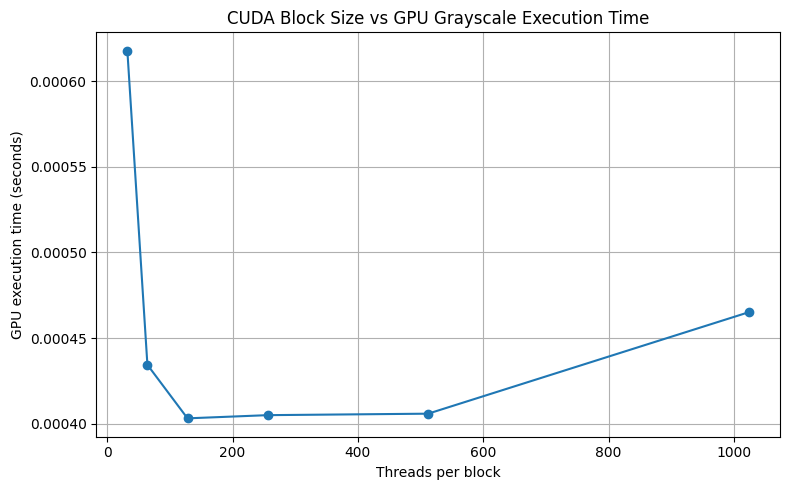
\includegraphics[width=0.8\textwidth]{block_size_vs_time.png}
\caption{CUDA block size versus GPU grayscale execution time}
\label{fig:block-size}
\end{figure}

The results show that a block size of 32 threads gives the highest execution time among the tested configurations, at 0.000618 seconds. Increasing the block size to 64 and 128 threads significantly reduces the execution time.

The lowest measured execution time is obtained with 128 threads per block, at approximately 0.000403 seconds. The results for 256 and 512 threads are very close, with execution times of 0.000405 and 0.000406 seconds respectively.

When the block size is increased to 1024 threads, the execution time increases to 0.000465 seconds. This shows that increasing the number of threads per block does not always improve performance. The GPU architecture must balance the number of active threads, scheduling, resource usage, and the number of blocks.

For this particular experiment, 128 threads per block produced the lowest measured execution time. However, the difference between 128, 256, and 512 threads is very small, so these configurations have similar performance for this workload.

\section{Discussion}

The experiment demonstrates the benefit of parallel execution for a highly parallel image-processing operation. Each pixel can be processed independently, making the grayscale conversion well suited to GPU execution.

The CPU implementation processes pixels sequentially, while the CUDA implementation distributes the pixel calculations among many GPU threads. This results in a substantially lower kernel execution time on the GPU.

The block-size experiment also demonstrates that CUDA performance depends on the selected execution configuration. Very small blocks can increase the number of blocks that must be scheduled, while very large blocks do not necessarily provide better performance. In this experiment, 128 threads per block achieved the lowest measured execution time, while 256 and 512 threads produced almost identical results.

Because the measured GPU execution times are very small, differences between nearby configurations can also be affected by measurement noise and system conditions. Therefore, the experiment should be interpreted as a measurement of this particular workload on the available GPU rather than a universal rule that 128 threads is always optimal.

\section{Conclusion}

This labwork successfully implements an RGB-to-grayscale image converter using both CPU and CUDA GPU computation.

The image was loaded from a file, converted into a flattened RGB array, and processed using the grayscale formula:

$$
Gray = 0.299R + 0.587G + 0.114B
$$

The GPU implementation produced results equivalent to the CPU implementation while achieving a measured kernel speedup of approximately 3336.63$\times$ compared with the sequential CPU implementation.

The block-size experiment showed that CUDA execution performance depends on the number of threads per block. Among the tested configurations, 128 threads per block achieved the lowest measured execution time of 0.000403 seconds. The experiment demonstrates the importance of selecting an appropriate CUDA execution configuration for GPU performance.


\end{document}